\chapter{Method}
\section{Choice of Method}
\begin{figure}[h]
%\hspace*{-0.4cm}
\begin{center}
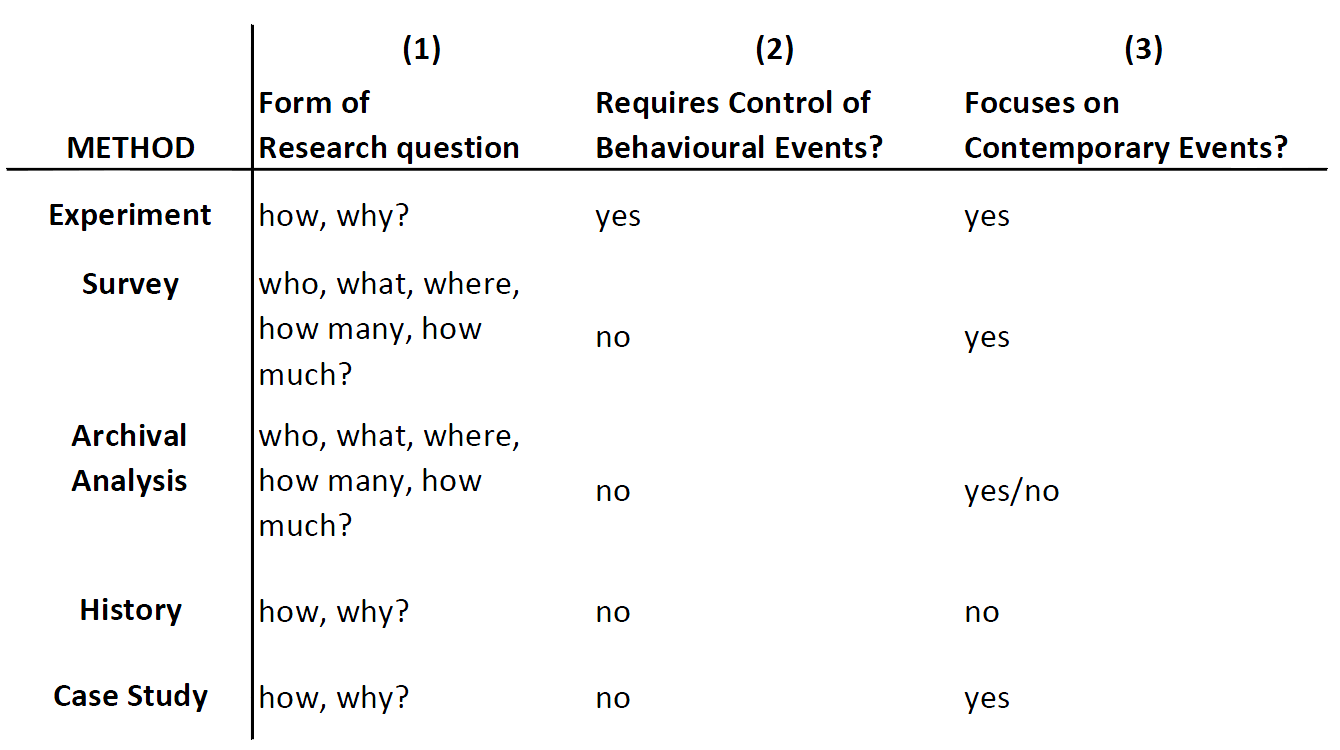
\includegraphics[scale=0.35]{methods.png}
\caption[Situations for different research methods]{Situations for different research methods, derived from \cite{CaseStudyResearch}}
\label{fig:methods}
\end{center}
\end{figure}
\section{Case Study}
%\cite{CaseStudyResearch}
%\cite{kitchenham1995case}
\subsection{Why Case Study?}

\subsection{Background Study}
The first step in our research were a background study of security incident management. In order to find appropriate questions for the interviews we found it necessary to study relevant literature such as standards and best practice guidelines. We focused on the well-established and internationally accepted ISO/IEC standards in addition to documentation from the \ac{NIST}.

We also looked at related work and what have been studied earlier in the field of incident management. 

Also had to study ``case study" techniques.

\subsection{Qualitative research}
We used a qualitative research method where we focused on relatively few informants. Unlike a quantitative approach where using questionnaires to gather information from a large number of participants is common, we wanted in-depth information from selected organizations. This eliminated the possibility to generalize results, but gave us more exhaustive answers and thus better suited data for our research.

\subsection{Qualitative Interviews}
We chose to perform qualitative interviews in our research as they are known as common and powerful tools to gather information in qualitative research\cite{myers2007qualitative}. The goal of qualitative interviews is to see the research topic from the interviewee's perspective and understand why and how they got that particular perspective\cite{cassell2004essential}. To meet this goal, qualitative interviews are driven by open questions and a low degree of structure and often focus on specific situations and experiences made by the interviewee. 

We used what is referred to in literature as semi-structured interviews\cite{cassell2004essential}. We wanted interviewees to talk freely about their experiences, and thus we did not follow a strict list of predefined questions. However, to ensure we got all information required to answer our research questions we used an interview guide. The interview guide works as an incomplete script and states the main goals for our research as well as the main research questions set up for the interview.

The interview questions were not asked in any particular order, but rather when found appropriate to ensure a smooth dialogue. This gave opportunities to ask follow-up questions. When using semi-structured interviews, interviewees can be seen as being ``participants" in the research, rather than someone who only answers pre-defined questions.

We performed the interviews face-to-face voice recorded the dialogue. By conducting interviews face-to-face we hoped to build trust with the interviewee and thus get better and more elaborative answers. It also gave us opportunity to explain and elaborate questions that were unclear. Since we recorded all of the interviews we could focus on listening and thus ask the best follow-up questions instead of being extracted by writing answers. Also, we could listen to the recordings several times as needed and clarify things that were unclear later.

Developing an interview guide, carrying out interviews and analysing them can be highly time-consuming activities. Participating in interviews is also time-consuming for interviewees, which could have made it challenging to recruit interviewees for our study. One mitigation to the risk of not recruiting interviewees was sending out letters explaining the main purpose of our research, what was expected by the interviewee, and how the interviews would play out. We also notified organizations at an early stage and set dates for the interviews to ensure their commitment.

Qualitative interviews are very flexible as they can be used to tackle various forms of research questions related to organizations. Despite the time effort spent on developing interview guides, questions and conducting the interviews, we found qualitative interviews to add great value and thus the most suited for our research.


\subsection{Participants}
In the nature of qualitative research participants were chosen to be diverse such that different perspectives on incident management (in the same context) could be studied.
large organizations that are likely to have experiences severe security incidents. + de i gjørvik gjorde på small/medium.. her gjør vi en dybdestudie av noe annet!

Hvorfor de vi valgte?

\subsection{Document study}
%\subsection{Action Research}
\section{Ethical Considerations}
%Litt i forhold til at man behandler sensitiv information og sånn
\subsection{Anonymization}
\section{Challenges}

